\section{Model}
\label{sec:model}

\subsection{The repeated market}

Time is discrete, $t=1,2,\dots$ Each period a fresh asset value
$v_t$ is drawn i.i.d.\ with mean $\bar v$ (normalised to $0$) and variance
$\sigma_v^2$. $I\ge 2$ learning informed traders observe $v_t$ and submit
market orders $x_{i,t}$. Noise traders submit $u_t\sim\mathcal N(0,\sigma_u^2)$,
and $P\ge 0$ optional \emph{passive} informed traders play a fixed Nash
strategy. Following \citet{dou2025}, a mass $\xi\ge0$ of
information-insensitive investors demands $z_t=-\xi(p_t-\bar v)$. A market
maker observes aggregate informed and noise flow $y_t=\sum_i x_{i,t}+u_t$ and
sets
\begin{equation}
  p_t=\arg\min_p\; \theta\,\big(p-\mathbb E[v_t\mid y_t]\big)^2+(y_t+z_t)^2
  \quad\Longrightarrow\quad
  p_t=\bar v+\lambda y_t,\qquad
  \lambda=\frac{\theta\lambda_B+\xi}{\theta+\xi^2},
  \label{eq:lambda}
\end{equation}
where $\lambda_B=\mathrm{Cov}(v,y)/\mathrm{Var}(y)$ is the Bayesian price impact.
With $\xi=0$ this is the \citet{kyle1985} market maker. Trader $i$ earns
$\pi_{i,t}=(v_t-p_t)\,x_{i,t}$. The value is revealed at the end of the period,
and the one-period game repeats.

\subsection{Benchmarks}

With linear strategies $x_i=\beta_i v$, profits depend only on second moments,
so the benchmarks below hold for any value distribution as long as pricing is
linear. Let $n=I+P$.

\begin{proposition}[Nash and collusive benchmarks]\label{prop:bench}
Let $\xi=0$. The symmetric Nash equilibrium of the stage game has
$\beta^N=\sigma_u/(\sqrt n\,\sigma_v)$ and $\lambda^N=\sqrt n\,\sigma_v/((n+1)\sigma_u)$.
If the learners jointly maximise their profit against a market maker who prices
their joint strategy rationally, while passive traders keep playing
$\beta^N$ (aggregate $B_P=P\beta^N$), the learners' aggregate intensity is
\[
B_L^{C}=\sqrt{B_P^2+\sigma_u^2/\sigma_v^2}.
\]
For $\xi>0$, the Nash intensity solves $\beta=1/\big((n+1)\lambda(n\beta)\big)$,
which has a unique root, and the collusive intensity maximises
$B_L\sigma_v^2\big(1-\lambda(B_L+B_P)\,(B_L+B_P)\big)$.
\end{proposition}

Collusion lowers aggregate intensity ($B_L^C<I\beta^N$ for $P=0$), raises
learners' profit, and reduces price informativeness
$\mathcal I=\mathrm{Corr}(p,v)^2=B^2\sigma_v^2/(B^2\sigma_v^2+\sigma_u^2)$.
Following \citet{calvano2020} we report any outcome metric $m$ as a
\emph{collusion index}
\[
\Delta_m=\frac{m-m^N}{m^C-m^N},
\]
so $\Delta=0$ is competition and $\Delta=1$ is the cartel. We use aggregate
intensity (the estimated slope of learners' total order on $v$),
informativeness, and profit. Because the Nash--cartel profit gap is only
$6\%$ at $I=2$, intensity and informativeness are the more precise measures.

\begin{remark}[Passive traders can remove the gain from collusion]
With $\xi=0$ and $\sigma_v=\sigma_u$, $B_L^C=\sqrt{P^2/n+1}$ and
$I\beta^N=I/\sqrt n$, which coincide exactly when $I=P+1$. In that case the
learners have nothing to gain from colluding and $\Delta$ is undefined. We avoid
this ratio when using passive traders as an intervention.
\end{remark}

\subsection{How detectable is a deviation?}

Punishment requires monitoring. The relevant quantity is how much a deviation
moves what traders observe relative to noise. Suppose rivals play the collusive
intensity and the market maker prices at $\lambda^C$. A trader's myopic best
response is $\beta^d=(1-\lambda^C (I-1)\beta^C)/(2\lambda^C)$, and a one-period
deviation moves aggregate flow by $(\beta^d-\beta^C)v$ against noise of
standard deviation $\sigma_u$.

\begin{proposition}[Deviation signal-to-noise]\label{prop:snr}
Let $P=0$ and define $\mathrm{SNR}=(\beta^d-\beta^C)\sigma_v/\sigma_u$, the
flow change of a best-response deviation per unit of $v/\sigma_v$, in noise
standard deviations.
\begin{enumerate}
\item If $\xi=0$, $\mathrm{SNR}=(I-1)/(2I)<1/2$ for all $I$, independently of
$\sigma_u$ and $\sigma_v$.
\item As $\xi\to\infty$ with $\theta$ fixed, $\mathrm{SNR}=\xi\sigma_v(I-1)/(4I\sigma_u)\,(1+o(1))$.
\end{enumerate}
\end{proposition}

\begin{figure}[t]
  \centering
  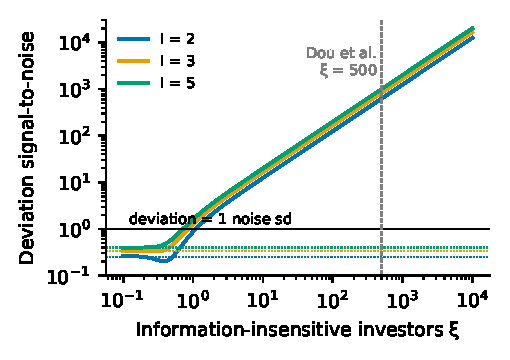
\includegraphics[width=0.55\linewidth]{figures/fig_snr.pdf}
  \caption{Signal-to-noise ratio of a one-period best-response deviation from
  the collusive intensity (order-flow change per unit of $v/\sigma_v$, in noise
  standard deviations), as a function of the mass of information-insensitive
  investors ($\sigma_v=1$, $\sigma_u=0.1$, $\theta=0.1$). Dotted lines: the
  $\xi=0$ values $(I-1)/(2I)$. Deviations become visible above noise only once
  $\xi$ exceeds about one; at the \citet{dou2025} calibration they are several
  hundred noise standard deviations large.}
  \label{fig:snr}
\end{figure}

\noindent The proof is in Appendix~\ref{app:proofs}; Figure~\ref{fig:snr}
plots the exact ratio. In the standard Kyle
market every intensity scales with $\sigma_u/\sigma_v$, so changing noise
volume rescales deviations and noise alike and cannot make monitoring easier. A
single deviation is less than half a noise standard deviation even at
$|v|=\sigma_v$, so a trigger strategy tuned to catch it would mostly fire on
noise. With information-insensitive investors, price impact is pinned near
$1/\xi$, intensities scale with $\xi$, and deviations become enormous relative
to noise: in the \citet{dou2025} calibration ($\sigma_v=1$, $\sigma_u=0.1$,
$\xi=500$, $\theta=0.1$, $I=2$) the ratio is about $625$. Detectability
therefore predicts exactly the regime split that \citet{dou2025} report:
over-pruning only at $\xi=0$, price triggers at $\xi=500$.
